\documentclass[border=4pt]{standalone}
\usepackage{tikz}
\usetikzlibrary{arrows,arrows.spaced,positioning}
\begin{document}
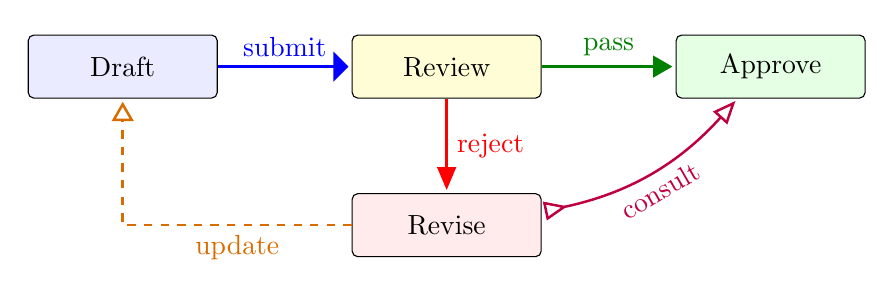
\begin{tikzpicture}[
  node distance=12mm and 17mm,
  stage/.style={draw,rounded corners=2pt,minimum width=24mm,minimum height=8mm,align=center},
  route/.style={line width=.9pt}
]
  \node[stage,fill=blue!8] (draft) {Draft};
  \node[stage,fill=yellow!16,right=of draft] (review) {Review};
  \node[stage,fill=green!10,right=of review] (approve) {Approve};
  \node[stage,fill=red!8,below=of review] (revise) {Revise};

  \draw[route,blue,-{spaced triangle 90}]
    (draft) -- node[above]{submit} (review);
  \draw[route,green!50!black,-{spaced triangle 60}]
    (review) -- node[above]{pass} (approve);
  \draw[route,red,-{spaced triangle 45}]
    (review) -- node[right]{reject} (revise);
  \draw[route,dashed,orange!85!black,-{spaced open triangle 60}]
    (revise.west) -| node[pos=.25,below]{update} (draft.south);
  \draw[route,purple,{spaced open triangle 45 reversed}-{spaced open triangle 45}]
    (revise) to[bend right=18] node[below,sloped]{consult} (approve);
\end{tikzpicture}
\end{document}
